% Informe de avance (pasos 1 y 2). Compilar desde esta carpeta:  latexmk -pdf reporte.tex
% Figuras y tablas se leen de ../resultados/paso2/ (generadas por paso2_features.py y material_reporte.py).
\documentclass[11pt,a4paper]{article}

\usepackage[T1]{fontenc}
\usepackage{lmodern}
\usepackage[english,spanish,es-noshorthands,es-tabla]{babel}  % el último es el idioma principal
\usepackage[margin=2.5cm]{geometry}
\usepackage{microtype}
\usepackage{amsmath}
\usepackage{booktabs}
\usepackage{tabularx}
\usepackage{graphicx}
\usepackage{xcolor}
\usepackage{tikz}
\usetikzlibrary{positioning,arrows.meta}
\usepackage{siunitx}
\sisetup{output-decimal-marker={,}}
\usepackage[font=small,labelfont=bf]{caption}
\usepackage{placeins}            % \FloatBarrier: que una tabla no pase a la sección siguiente
\usepackage[autostyle]{csquotes}
\usepackage{babelbib}            % bibliografía con BibTeX y textos fijos en español (estilo babunsrt-lf)
\selectbiblanguage{spanish}
\usepackage{cite}
\usepackage[hidelinks]{hyperref}

\graphicspath{{../resultados/paso2/}}
\makeatletter  % \input primitivo: expandible, así \bottomrule puede seguir a las filas leídas del archivo
\newcommand{\tabla}[1]{\@@input ../resultados/paso2/tablas/#1 }
\makeatother
\newcommand{\uV}{\si{\micro\volt}}
\definecolor{azul}{HTML}{2A78D6}
\definecolor{gris}{HTML}{52514E}

\title{Efecto de la longitud de ventana y del solapamiento\\en la extracción de características EEG\\[6pt]
  \large TEPT, enfermedad de Alzheimer y depresión mayor\\Informe de avance: datos, procesamiento y estabilidad}
\author{Aldrin Josue Chavez Piguave \and Jhony Alfonso Peñaherrera Loor \and
        Marck Anthony Chiza Segovia \and Fernando Chalanero Chantera Matango}
\date{24 de noviembre de 2026}

\begin{document}
\maketitle

\begin{abstract}
El artículo OnTEPT integra características EEG de pacientes con trastorno de estrés postraumático (TEPT), pero no documenta con qué parámetros se calcularon ni qué tan fiables son. Este trabajo exploratorio estudia cómo la longitud de ventana (1, 2 y 4~s) y el solapamiento (0, 50 y 75~\%) afectan a la extracción de características EEG en tres enfermedades. Se seleccionaron tres conjuntos de datos públicos: TEPT (6 pacientes y 6 controles), enfermedad de Alzheimer (36 y 29) y depresión mayor (28 y 27). Todas las señales se armonizaron con el mismo procesamiento (19 canales, 256~Hz, 1--40~Hz, referencia promedio, 240~s por sujeto y rechazo de artefactos), y de cada ventana se extrajeron 228 características: potencia absoluta y relativa en cinco bandas, entropía espectral y entropía de permutación. La estabilidad entre la primera y la segunda mitad de cada registro fue alta en las nueve configuraciones (ICC mediano entre 0,93 y 0,96): el solapamiento no la modificó y la longitud de ventana apenas lo hizo. En cambio, el solapamiento multiplicó el tiempo de cálculo (unas 2 veces con 50~\% y unas 7 con 75~\%), y las ventanas largas perdieron más datos por artefactos. Queda pendiente la interpretación de modelos con SHAP.
\end{abstract}

% ---------------------------------------------------------------------------------------------
\section{Introducción}

OnTEPT~\cite{salazar2026} es una ontología OWL que formaliza los criterios diagnósticos del TEPT según el DSM-5 y la CIE-11 e integra datos psicométricos y de EEG. Su versión actual codifica 36 características EEG cuantitativas (estadísticas, espectrales, de entropía y de asimetría) de 41 participantes. Sin embargo, el artículo no documenta con qué parámetros se calcularon esas características, como la longitud de ventana o el solapamiento, ni qué tan fiables son. Sus propios autores señalan la heterogeneidad de los protocolos de adquisición como una de las razones para no formalizar todavía reglas diagnósticas basadas en EEG.

Este trabajo extiende la pregunta más allá del TEPT. Es un análisis exploratorio de investigación, no un sistema clínico. La pregunta es: \emph{¿cómo cambian la estabilidad, el costo de cálculo y la relevancia de las características EEG según la longitud de ventana y el solapamiento?} Los objetivos son:
\begin{enumerate}
  \item Seleccionar tres conjuntos de datos públicos de EEG: uno de TEPT y dos de otras enfermedades neurológicas o psiquiátricas.
  \item Comparar nueve configuraciones de extracción (ventanas de 1, 2 y 4~s por solapamientos de 0, 50 y 75~\%) en estabilidad y tiempo de procesamiento.
  \item Entrenar, en cada conjunto de datos por separado, un clasificador simple de pacientes frente a controles con validación cruzada por sujeto, e interpretar con SHAP qué características, bandas y canales pesan más en cada configuración.
\end{enumerate}

Una regla de diseño atraviesa todo el trabajo: los conjuntos de datos no se mezclan en un mismo modelo. Cada uno se registró con un equipo distinto, y un modelo conjunto podría aprender a reconocer el equipo en lugar de la enfermedad. Este informe cubre los objetivos 1 y 2; el objetivo 3 está pendiente (sección~\ref{sec:pendiente}).

% ---------------------------------------------------------------------------------------------
\section{Datos}

\subsection{Criterios de selección}
Se buscaron conjuntos de datos que cumplieran, en lo posible: acceso abierto, diagnóstico etiquetado, grupo de controles sanos, registro en reposo y canales y frecuencia de muestreo documentados. Todos los enlaces y metadatos se verificaron directamente en cada repositorio el 24 de noviembre de 2026.

\subsection{Revisión de las fuentes de EEG citadas por OnTEPT}
\begin{itemize}
  \item \textbf{du Bois et al.}~\cite{dubois2022}: 29 mujeres con TEPT, sobrevivientes del genocidio de 1994 en Ruanda, asignadas a un grupo control (9), uno de imaginación motora (10) y uno de neurorretroalimentación (10). El \enquote{grupo control} está formado por pacientes con TEPT sin intervención, no por personas sanas. Además, según la tabla~1 de ese artículo, el grupo control no tiene EEG: hay registros de 20 participantes. Este conjunto no permite comparar pacientes con controles.
  \item \textbf{Rahmani et al.}~\cite{rahmani2018}: 6 pacientes con TEPT de combate y 6 controles. Es la única fuente con controles sanos. La declaración de disponibilidad de datos de OnTEPT enlaza un DOI equivocado para este conjunto (\texttt{10.1371/journal.pone.0282001}, que corresponde a un estudio sobre hipertensión en personas con VIH); los datos están en figshare~\cite{rahmani2018datos}.
  \item \textbf{DAIC-WOZ}: solo aporta respuestas al cuestionario PCL-C; no contiene EEG.
\end{itemize}
Con estos datos, OnTEPT tendría registros EEG de 32 participantes (20 + 12), no de 41.

\subsection{Otras fuentes revisadas}
No se encontró en OpenNeuro ningún conjunto de EEG de TEPT (búsquedas por \emph{PTSD}, \emph{posttraumatic} y \emph{trauma}). TDBRAIN~\cite{vandijk2022} no incluye TEPT y exige registro con ORCID y un acuerdo de uso de datos. Park et al.~\cite{park2021} incluyen 52 pacientes con TEPT y 95 controles, pero solo publican características ya calculadas (un CSV de 945 sujetos y 1\,149 columnas de potencia y coherencia), sin señal cruda, de modo que no permiten probar configuraciones de ventana. Para las otras enfermedades se evaluaron también conjuntos de esquizofrenia (RepOD) y de enfermedad de Parkinson (OpenNeuro ds004584 y ds002778).

\subsection{Conjuntos de datos seleccionados}
La tabla~\ref{tab:datasets} resume los tres conjuntos elegidos. Difieren en casi todo: lugar, equipo, población, frecuencia de muestreo, referencia, duración y procesado previo. Esa heterogeneidad es la que obliga a armonizar las señales (sección~\ref{sec:armonizacion}) y a entrenar un modelo por conjunto.

\begin{table}[ht]
\centering\small
\caption{Conjuntos de datos seleccionados.}
\label{tab:datasets}
\begin{tabular}{@{}>{\raggedright\arraybackslash}p{2.4cm} *{3}{>{\raggedright\arraybackslash}p{4.1cm}}@{}}
\toprule
 & TEPT & Alzheimer & Depresión mayor \\
\midrule
Fuente & Rahmani et al.~\cite{rahmani2018,rahmani2018datos} & Miltiadous et al.~\cite{miltiadous2023,openneuro2026ds004504} & Mumtaz et al.~\cite{mumtaz2017,mumtaz2016datos} \\
Lugar & Laureate Institute for Brain Research (EE.\,UU.) & Hospital AHEPA, Tesalónica (Grecia) & Universiti Sains Malaysia (Malasia) \\
Participantes & 6 TEPT de combate y 6 controles; varones, $27 \pm 5$ años & 36 Alzheimer y 29 controles (se excluyen 23 con demencia frontotemporal); edad media 66 y 68 años & 34 con depresión mayor (DSM-IV) y 30 controles en el repositorio\textsuperscript{a} \\
Registro & Dentro del resonador, simultáneo con fMRI; condición no documentada & Nihon Kohden EEG 2100; reposo, ojos cerrados & Brain Master Discovery 24e; reposo, ojos cerrados \\
Canales & 31 EEG + ECG & 19 & 19 + 2--3 auxiliares \\
Muestreo & 250 Hz & 500 Hz & 256 Hz \\
Referencia original & FCz & Cz\textsuperscript{b} & Orejas unidas \\
Duración & 520 s & 5--21 min & $\approx$ 5 min \\
Procesado previo & Sí: artefactos del resonador eliminados, filtro a 40 Hz e ICA & No & No \\
Formato y licencia & Texto; CC BY 4.0 & EEGLAB (BIDS); CC0 & EDF; CC BY 4.0 \\
\bottomrule
\end{tabular}

\smallskip
\raggedright\footnotesize
\textsuperscript{a} No todos son utilizables; la muestra final está en la tabla~\ref{tab:muestra}.
\textsuperscript{b} Según la descripción del conjunto; sus metadatos BIDS indican A1--A2.
\end{table}

\subsection{Control de calidad y muestra final}
\begin{itemize}
  \item Seis archivos de ojos cerrados del conjunto de depresión no se pueden descargar: figshare los lista sin huella MD5 y sus enlaces devuelven errores 403/404 (controles S12 y S18; pacientes S4, S8, S12 y S16).
  \item Hay dos pares de archivos idénticos byte a byte con nombres distintos (H\_S27 = H\_S30 y MDD\_S33 = MDD\_S34). Se conserva el de número menor. Si una copia quedara en entrenamiento y la otra en prueba, el clasificador reconocería la señal y no la enfermedad. El procesamiento detecta duplicados en todos los conjuntos comparando una huella MD5 de la señal.
  \item Un registro (MDD\_S3, 180~s) es más corto que la duración común de 240~s y se excluye.
  \item En el conjunto de depresión, 22 de 28 archivos de controles traen dos canales auxiliares que solo aparecen en 1 de 30 archivos de pacientes. Solo se usan los 19 canales comunes, para que el formato del archivo no delate el grupo.
\end{itemize}
La muestra final tiene 132 sujetos (tabla~\ref{tab:muestra}).

\begin{table}[ht]
\centering\small
\caption{Muestra final y porcentaje de segundos descartados por artefactos (mediana por grupo). \enquote{Disponibles}: registros descargados.}
\label{tab:muestra}
\begin{tabular}{@{}llrrr@{}}
\toprule
Conjunto & Grupo & Disponibles & Incluidos & Segundos descartados (\%) \\
\midrule
\tabla{muestra.tex}
\bottomrule
\end{tabular}
\end{table}

% ---------------------------------------------------------------------------------------------
\section{Métodos}

La figura~\ref{fig:pipeline} resume el procesamiento. Todo se implementó en Python con NumPy, SciPy~\cite{virtanen2020} y MNE~\cite{gramfort2013}. Los pasos de armonización son idénticos para los tres conjuntos.

\begin{figure}[ht]
\centering
\begin{tikzpicture}[
    caja/.style={draw=azul, fill=azul!7, rounded corners=2pt, align=center, font=\footnotesize,
                 minimum height=12mm, text width=20mm, inner sep=2pt},
    analisis/.style={caja, draw=gris, fill=gris!6},
    flecha/.style={-{Stealth[length=2mm]}, semithick, draw=gris},
    node distance=8mm and 4mm]
  \node[caja] (a) {Lectura: 19 canales en \uV};
  \node[caja, right=of a] (b) {Remuestreo a 256 Hz};
  \node[caja, right=of b] (c) {Filtro 1--40 Hz};
  \node[caja, right=of c] (d) {Referencia promedio};
  \node[caja, right=of d] (e) {Recorte a 240 s};
  \node[caja, right=of e] (f) {Segundos con artefactos};
  \node[analisis, below=of f] (g) {Ventanas: 9 configuraciones};
  \node[analisis, left=of g] (h) {228 características por ventana};
  \node[analisis, left=of h] (i) {Estabilidad (ICC) y tiempo};
  \node[analisis, left=of i, dashed] (j) {Clasificador y SHAP (pendiente)};
  \foreach \x/\y in {a/b, b/c, c/d, d/e, e/f, f/g, g/h, h/i, i/j}
    \draw[flecha] (\x) -- (\y);
\end{tikzpicture}
\caption{Flujo del análisis. Fila superior: armonización de la señal, idéntica para los tres conjuntos. Fila inferior: segmentación, características y evaluación.}
\label{fig:pipeline}
\end{figure}

\subsection{Armonización y preprocesamiento}
\label{sec:armonizacion}
La tabla~\ref{tab:preproc} detalla cada paso y su justificación. Conviene distinguir dos sentidos de \enquote{estandarizar}. Aquí se armoniza la \emph{señal}, es decir, se lleva a los tres conjuntos al mismo formato. La estandarización de las \emph{características} (media cero y varianza uno) se hará en el paso~3, dentro de la validación cruzada y ajustada solo con los sujetos de entrenamiento; calcularla con todos los sujetos filtraría información del conjunto de prueba.

\begin{table}[ht]
\centering\small
\caption{Pasos de armonización, idénticos para los tres conjuntos de datos.}
\label{tab:preproc}
\begin{tabularx}{\textwidth}{@{}>{\raggedright\arraybackslash}p{1.9cm} >{\raggedright\arraybackslash}X >{\raggedright\arraybackslash}X@{}}
\toprule
Paso & Qué se hace & Por qué \\
\midrule
Canales & 19 electrodos del sistema 10-20 (Fp1, Fp2, F7, F3, Fz, F4, F8, T3, C3, Cz, C4, T4, T5, P3, Pz, P4, T6, O1, O2). En Rahmani, T7, T8, P7 y P8 se renombran T3, T4, T5 y T6 & Son los únicos presentes en los tres conjuntos; los nombres de Rahmani son la nomenclatura 10-10 de los mismos puntos \\
Unidades & Microvoltios (\uV) & Misma escala en todos. Para Rahmani, que no indica la unidad, se asume \uV\ por la resolución que reporta su artículo \\
Muestreo & 256 Hz, con remuestreo polifásico y filtro antialias & La entropía de permutación depende de la frecuencia de muestreo. Con 256 Hz todos los avances de ventana son enteros (a 250 Hz, 1~s con 75~\% serían 62,5 muestras) \\
Filtro & Pasa-banda de 1 a 40 Hz, Butterworth de orden 4 aplicado hacia adelante y hacia atrás (fase cero) & Quita derivas lentas. El techo de 40 Hz lo impone Rahmani, ya filtrado así; además elimina la red eléctrica (50/60 Hz) \\
Referencia & Promedio de los 19 canales & Cada conjunto usaba otra referencia (FCz, Cz, orejas); con el promedio, la original se cancela \\
Duración & Segundos 1 a 241 de cada registro (240 s) & Misma cantidad de datos y mismo peso por sujeto; el primer segundo tiene efectos de borde del filtro \\
Artefactos & Un segundo es \enquote{malo} si algún canal supera \SI{150}{\micro\volt} pico a pico; se descartan las ventanas que lo tocan & Elimina parpadeos y movimientos sin descartar ritmo alfa amplio \\
\bottomrule
\end{tabularx}
\end{table}

El remuestreo y el filtrado se aplican al registro completo antes de recortar. El umbral de artefactos se eligió tras comparar 100, 150, 200 y 300~\uV: con 100~\uV\ se descartaba hasta el 32~\% de los segundos de algunos controles del conjunto de depresión cuya actividad normal es muy amplia (mediana de pico a pico de 86--93~\uV), mientras que con 150~\uV\ la mediana descartada fue de 0 a 4~\% según el grupo (tabla~\ref{tab:muestra}). El rechazo por umbral no limpia la señal, como haría el análisis de componentes independientes (ICA); solo descarta tramos. El conjunto de Rahmani llega ya preprocesado por sus autores, y el procesamiento común se aplica encima: no es posible deshacer el previo. La figura~\ref{fig:ejemplo} muestra el efecto del preprocesamiento en un registro real.

\begin{figure}[ht]
\centering
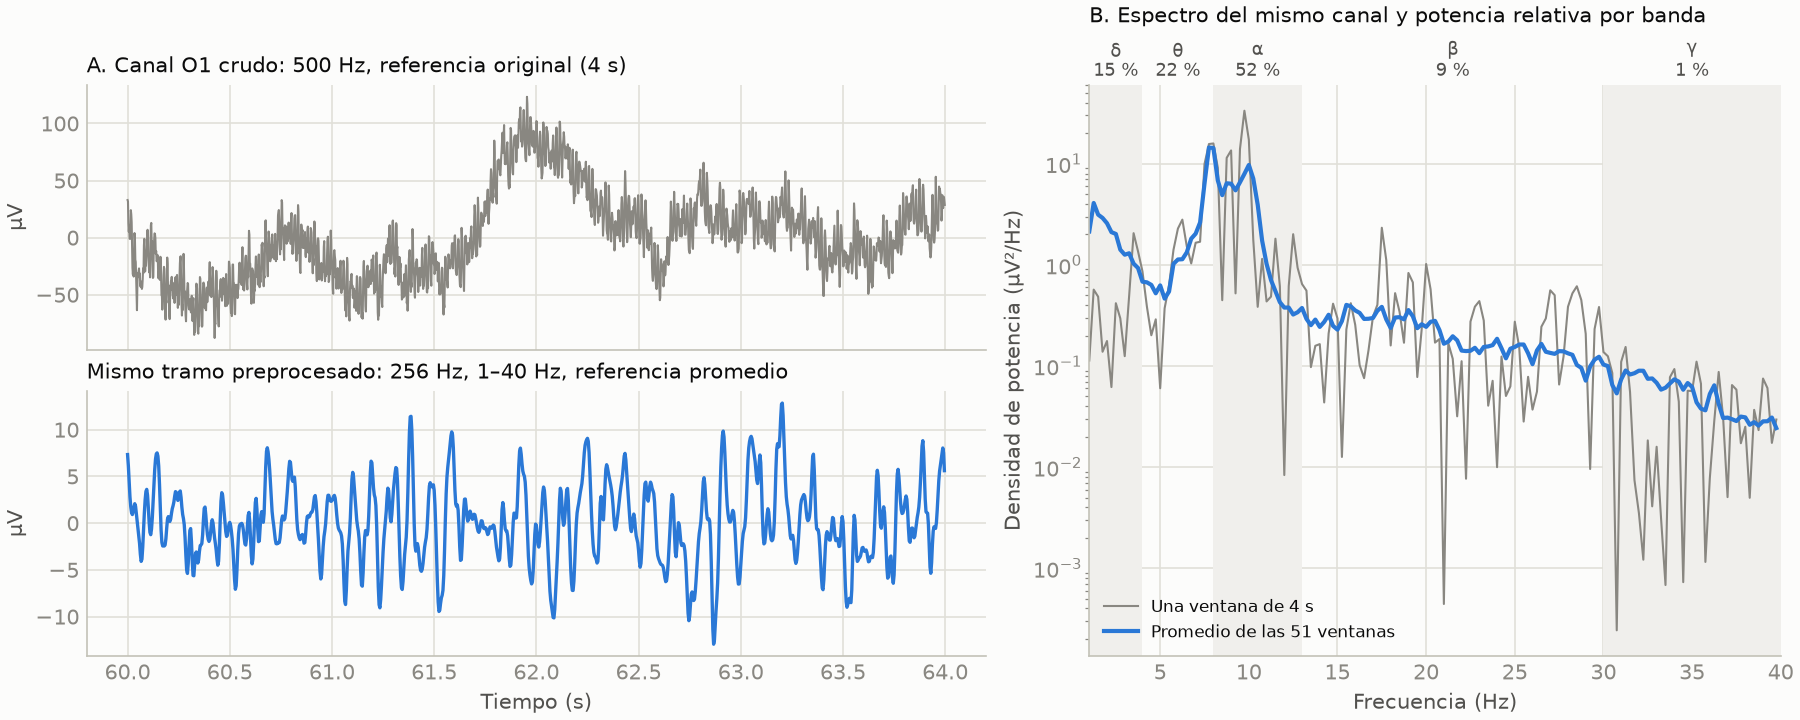
\includegraphics[width=\textwidth]{fig_ejemplo_senal.png}
\caption{Ejemplo con datos reales: control sub-050 de ds004504, elegido por tener la potencia relativa alfa mediana en O1 entre los controles. (A)~Cuatro segundos del canal O1, crudos y preprocesados: desaparecen la deriva lenta y el ruido de alta frecuencia, y aparece la oscilación cerebral. (B)~Espectro de una ventana de 4~s (gris) y promedio de las 51 ventanas limpias (azul); arriba, la potencia relativa de cada banda en el espectro promedio.}
\label{fig:ejemplo}
\end{figure}

\subsection{Segmentación en ventanas}
Cada registro armonizado (19 canales y 61\,440 muestras) se divide en ventanas de longitud $L \in \{1, 2, 4\}$~s con solapamiento $s \in \{0, 50, 75\}$~\%, es decir, con un avance de $L\,(1 - s)$ (tabla~\ref{tab:ventanas}). Dos consecuencias importan para la interpretación. Primera, el solapamiento aumenta el número de ventanas pero no la información: con 75~\%, cada muestra aparece en cuatro ventanas, que por tanto están muy correlacionadas. Segunda, la longitud fija la resolución en frecuencia, $\Delta f = 1/L$: con ventanas de 1~s la banda delta (1--4~Hz) se describe con solo 3 valores, y con 4~s, con 12.

\begin{table}[ht]
\centering\small
\caption{Configuraciones de ventana: muestras por ventana, avance y número de ventanas en 240~s antes de descartar artefactos.}
\label{tab:ventanas}
\begin{tabular}{@{}lrrrrrrr@{}}
\toprule
 & & \multicolumn{3}{c}{Avance (muestras)} & \multicolumn{3}{c}{Ventanas en 240 s} \\
\cmidrule(lr){3-5}\cmidrule(l){6-8}
Ventana & Muestras & 0 \% & 50 \% & 75 \% & 0 \% & 50 \% & 75 \% \\
\midrule
1 s & 256 & 256 & 128 & 64 & 240 & 479 & 957 \\
2 s & 512 & 512 & 256 & 128 & 120 & 239 & 477 \\
4 s & 1024 & 1024 & 512 & 256 & 60 & 119 & 237 \\
\bottomrule
\end{tabular}
\end{table}

\subsection{Características}
Para cada ventana y canal se calcula el periodograma con ventana de Hann, tras restar la media de la ventana, como densidad espectral de potencia $S(f_k)$ en \si{\micro\volt\squared\per\hertz}. Se usan cinco bandas: delta $[1, 4)$, theta $[4, 8)$, alfa $[8, 13)$, beta $[13, 30)$ y gamma $[30, 40)$~Hz; gamma queda limitada a 40~Hz por el filtro común. La potencia de una banda $b$ y las dos características derivadas son
\begin{equation}
  P_b = \sum_{f_k \in b} S(f_k)\,\Delta f, \qquad
  \mathrm{abs}_b = \log_{10} P_b, \qquad
  \mathrm{rel}_b = \frac{P_b}{\sum_{1 \le f_k < 40} S(f_k)\,\Delta f}.
\end{equation}
El logaritmo vuelve más simétrica la distribución de la potencia, que varía en órdenes de magnitud entre sujetos. La potencia relativa es un cociente, así que cancela la escala de amplitud (ganancia del equipo, impedancia, grosor del cráneo).

La entropía espectral~\cite{inouye1991} mide qué tan repartida está la potencia entre frecuencias. Vale 0 si toda la potencia está en una frecuencia y 1 si está repartida por igual:
\begin{equation}
  H_S = -\frac{1}{\ln K} \sum_{k=1}^{K} p_k \ln p_k, \qquad p_k = \frac{S(f_k)}{\sum_{j=1}^{K} S(f_j)},
\end{equation}
donde $K$ es el número de frecuencias en $[1, 40)$~Hz: 39, 78 o 156 para ventanas de 1, 2 o 4~s. Como $K$ depende de la ventana, los \emph{valores} de $H_S$ no son comparables entre longitudes de ventana distintas, aunque su estabilidad sí.

La entropía de permutación~\cite{bandt2002}, de orden 3 y retardo de una muestra, mide qué tan impredecible es la forma de onda. Se clasifica cada trío de muestras consecutivas $(x_t, x_{t+1}, x_{t+2})$ según su patrón de orden (hay $3! = 6$ posibles) y se calcula
\begin{equation}
  H_P = -\frac{1}{\ln 3!} \sum_{\pi} p(\pi) \ln p(\pi),
\end{equation}
donde $p(\pi)$ es la fracción de tríos con el patrón $\pi$. Una rampa da $H_P = 0$ y el ruido blanco, $H_P \approx 1$. La tabla~\ref{tab:features} resume las 12 características por canal; con 19 canales son 228 por ventana.

\begin{table}[ht]
\centering\small
\caption{Características calculadas en cada ventana y canal.}
\label{tab:features}
\begin{tabularx}{\textwidth}{@{}l c c >{\raggedright\arraybackslash}X@{}}
\toprule
Familia & Tipos & ¿Depende de la amplitud? & Qué mide \\
\midrule
Potencia absoluta & 5 & Sí & Actividad en la banda ($\log_{10}$ de \si{\micro\volt\squared}) \\
Potencia relativa & 5 & No & Proporción de la potencia total de 1--40 Hz \\
Entropía espectral & 1 & No & Dispersión del espectro, entre 0 y 1 \\
Entropía de permutación & 1 & No & Irregularidad de la forma de onda, entre 0 y 1 \\
\bottomrule
\end{tabularx}
\end{table}

\subsection{Estabilidad}
Para cada sujeto, configuración y característica se promedian las ventanas limpias de la primera mitad del registro (0--120~s) y las de la segunda (120--240~s). Las ventanas que cruzan el segundo 120, que solo existen con solapamiento, no entran en este análisis. La consistencia entre mitades se mide con el coeficiente de correlación intraclase de acuerdo absoluto para una medida~\cite{mcgraw1996}:
\begin{equation}
  \mathrm{ICC}(A,1) = \frac{MS_R - MS_E}{MS_R + (k-1)\,MS_E + \frac{k}{n}\,(MS_C - MS_E)},
\end{equation}
con $n$ sujetos y $k = 2$ mitades; $MS_R$ es el cuadrado medio entre sujetos, $MS_C$ el cuadrado medio entre mitades y $MS_E$ el residual. Intuitivamente, el ICC compara cuánto se diferencian los sujetos entre sí con cuánto cambia cada uno entre sus dos mitades. A diferencia de una correlación, el acuerdo absoluto también penaliza un cambio sistemático entre mitades. Se interpreta con los umbrales de Koo y Li~\cite{koo2016}: pobre por debajo de 0,5; moderada entre 0,5 y 0,75; buena entre 0,75 y 0,9; excelente por encima de 0,9. Para que las diferencias entre configuraciones no se deban a cambios en la muestra, se usan los mismos sujetos en las nueve configuraciones: los que tienen al menos cinco ventanas limpias por mitad en todas. Cumplieron la condición todos los sujetos (12, 65 y 55).

\subsection{Costo computacional}
Se mide con un cronómetro de alta resolución (\texttt{time.perf\_counter}) el tiempo de segmentar y calcular las 228 características, por sujeto y configuración. El preprocesamiento es común a todas las configuraciones y se midió aparte: mediana de 0,04 a 0,47~s por sujeto según el conjunto. Equipo: 8 núcleos lógicos y 7,8~GB de RAM, con poca memoria libre durante la medición; Python 3.11.2, NumPy 2.4.6, SciPy 1.17.1 y MNE 1.13.2. Los tiempos sirven para comparar configuraciones entre sí, no como valores absolutos.

\subsection{Verificación}
Antes de procesar, el programa ejecuta pruebas automáticas y se detiene si alguna falla:
\begin{itemize}
  \item un seno de 10~Hz da potencia relativa alfa de 1,000 y entropía espectral de 0,17;
  \item el ruido blanco da entropías de 0,93 (espectral) y 0,999 (permutación);
  \item una rampa da entropía de permutación 0;
  \item el ICC reproduce el valor de 0,29 del ejemplo clásico de Shrout y Fleiss~\cite{shrout1979};
  \item una ventana que toca un segundo con artefactos se descarta.
\end{itemize}
Además, se comprobó que las 27 matrices de características (3 conjuntos por 9 configuraciones) no tienen valores faltantes y que contienen los sujetos y grupos esperados.

% ---------------------------------------------------------------------------------------------
\section{Resultados}

\subsection{Calidad de los datos}
La mediana de segundos descartados por artefactos fue baja en todos los grupos, de 0 a 4~\% (tabla~\ref{tab:muestra}); el conjunto de Alzheimer fue el más afectado, sobre todo en pacientes. Se observó una diferencia de amplitud entre grupos: el valor cuadrático medio (RMS) mediano de la señal preprocesada fue de 4,0~\uV\ en pacientes con TEPT frente a 7,8~\uV\ en sus controles, y de 5,3 frente a 8,0~\uV\ en depresión. En Alzheimer los grupos fueron similares (7,7 y 7,6~\uV).

\subsection{Estabilidad}
La estabilidad entre mitades fue alta en los tres conjuntos y en las nueve configuraciones (tabla~\ref{tab:estab}, figura~\ref{fig:icc}). El solapamiento prácticamente no la modificó. La longitud de ventana tuvo efectos pequeños; el mayor fue la caída de la entropía espectral en TEPT, de 0,88 con 1~s a 0,83 con 4~s (tabla~\ref{tab:icc_tipos}).

\begin{table}[ht]
\centering\small
\caption{Resumen de la estabilidad entre mitades. Los efectos son la mayor diferencia del ICC mediano de un tipo de característica entre configuraciones: entre los tres solapamientos con la ventana fija, o entre las ventanas de 1 y 4~s sin solapamiento.}
\label{tab:estab}
\begin{tabular}{@{}lcccc@{}}
\toprule
Conjunto & ICC mediano & Características & Efecto del & Efecto de pasar \\
 & (9 configuraciones) & con ICC $\ge$ 0,75 & solapamiento & de 1 a 4 s \\
\midrule
TEPT ($n = 12$) & 0,93--0,94 & 86,4--89,5 \% & 0,07 & 0,05 \\
Alzheimer ($n = 65$) & 0,94--0,95 & 98,7--99,1 \% & 0,01 & 0,01 \\
Depresión ($n = 55$) & 0,96 & 99,6 \% & 0,02 & 0,02 \\
\bottomrule
\end{tabular}
\end{table}

\begin{table}[ht]
\centering\small
\caption{ICC mediano (sobre los 19 canales) por tipo de característica y longitud de ventana, sin solapamiento.}
\label{tab:icc_tipos}
\begin{tabular}{@{}l *{9}{c}@{}}
\toprule
 & \multicolumn{3}{c}{TEPT} & \multicolumn{3}{c}{Alzheimer} & \multicolumn{3}{c}{Depresión} \\
\cmidrule(lr){2-4}\cmidrule(lr){5-7}\cmidrule(l){8-10}
Característica & 1 s & 2 s & 4 s & 1 s & 2 s & 4 s & 1 s & 2 s & 4 s \\
\midrule
\tabla{icc_tipos.tex}
\bottomrule
\end{tabular}
\end{table}

\begin{figure}[ht]
\centering
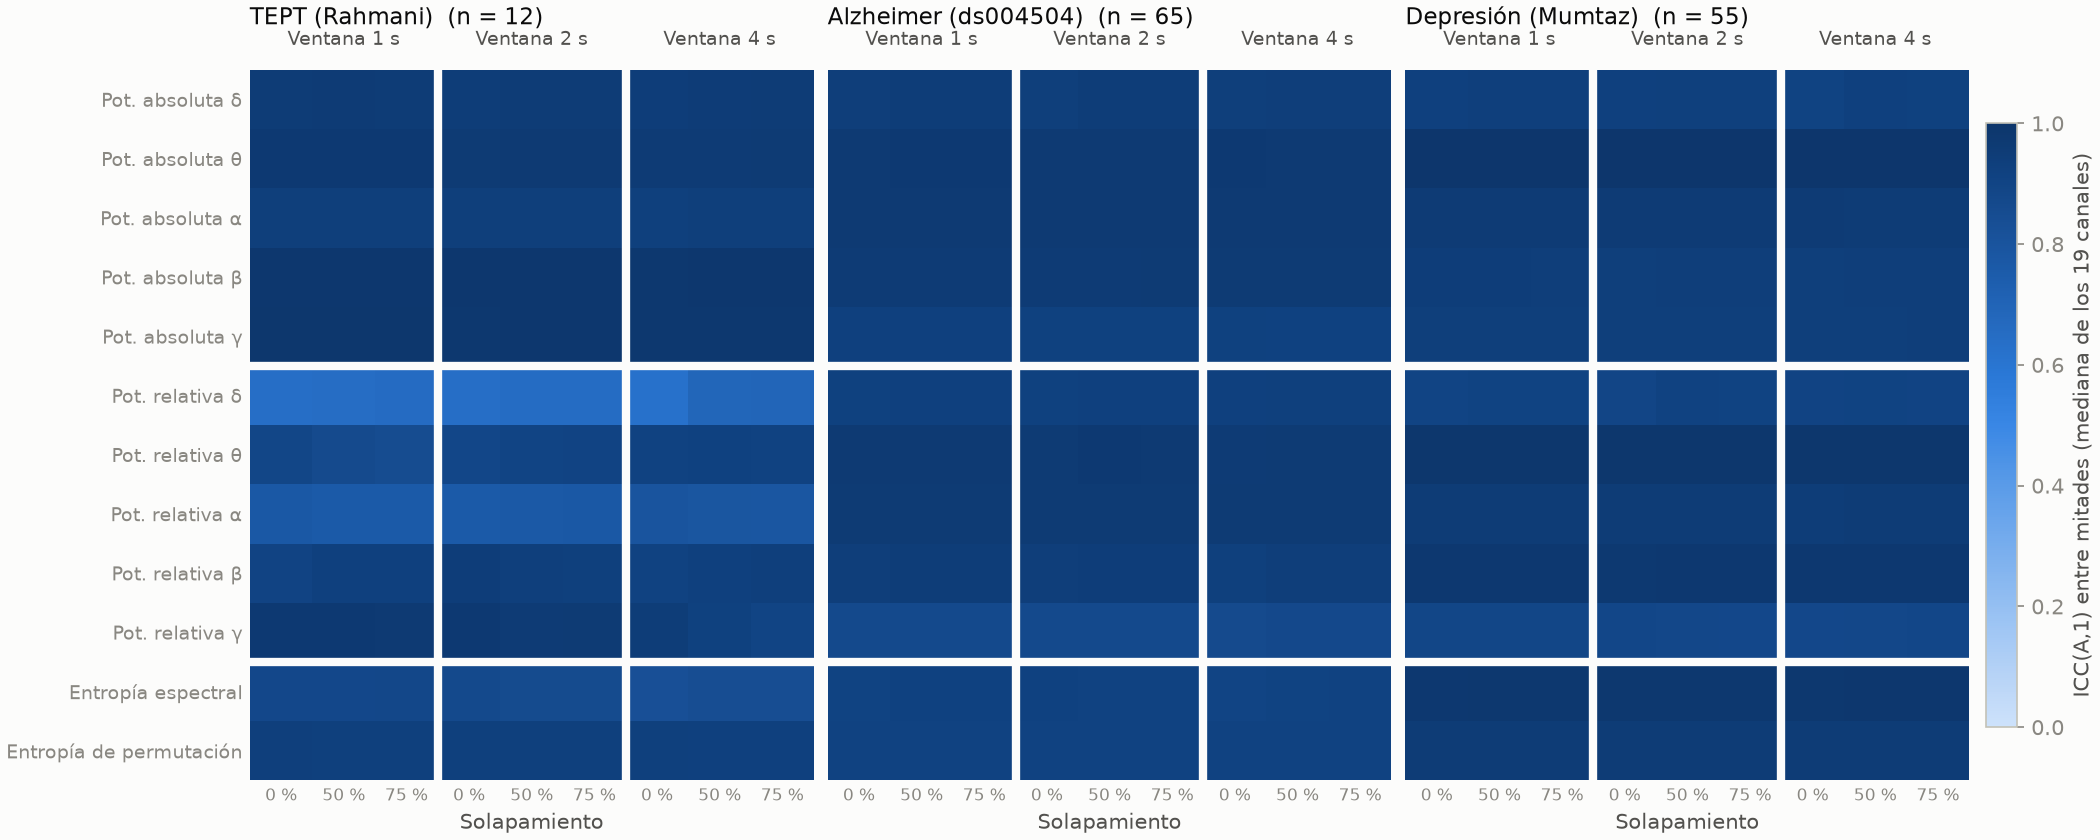
\includegraphics[width=\textwidth]{fig_estabilidad_icc.png}
\caption{ICC entre mitades (mediana de los 19 canales) para cada tipo de característica y configuración. Cuanto más oscuro, más estable.}
\label{fig:icc}
\end{figure}

Las características menos estables (ventana de 1~s, sin solapamiento) fueron:
\begin{itemize}
  \item Alzheimer y depresión: la potencia gamma relativa en canales frontales y temporales (ICC de 0,66 a 0,77; por ejemplo, F4 con 0,67 en Alzheimer y T3 con 0,66 en depresión). Es compatible con contaminación muscular en altas frecuencias, aunque no se ha comprobado.
  \item TEPT: la potencia relativa delta (mediana de 0,62 a 0,64) y alfa (0,76 a 0,79); la peor fue la alfa relativa en T4, con 0,10. En cambio, la potencia absoluta de TEPT fue muy estable (0,93 a 0,99). Una hipótesis, no verificada, son restos de artefactos del resonador en las bandas lentas.
\end{itemize}

\subsection{Costo computacional}
El tiempo por sujeto depende casi solo del solapamiento (tabla~\ref{tab:costo}, figura~\ref{fig:costo}). Sin solapamiento, cada muestra se procesa una vez, sea cual sea la longitud de ventana; con 50~\% se procesa dos veces y con 75~\%, cuatro. Se midió un factor de unas 2 veces con 50~\% y de unas 7 con 75~\%; el exceso sobre 4 probablemente se debe a la presión de memoria del equipo. El porcentaje de ventanas descartadas crece con la longitud de ventana, porque basta un segundo malo para descartar la ventana entera: en Alzheimer pasa del 4,8~\% con 1~s al 11,7~\% con 4~s.

\begin{table}[ht]
\centering\small
\caption{Costo por configuración: ventanas limpias y tiempo de extracción por sujeto (medianas de los 132 sujetos) y porcentaje de ventanas descartadas por artefactos en cada conjunto.}
\label{tab:costo}
\begin{tabular}{@{}llrrrrr@{}}
\toprule
 & & & & \multicolumn{3}{c}{Ventanas descartadas (\%)} \\
\cmidrule(l){5-7}
Ventana & Solapamiento & Ventanas/sujeto & Tiempo (ms) & TEPT & Alzheimer & Depresión \\
\midrule
\tabla{costo.tex}
\bottomrule
\end{tabular}
\end{table}

\begin{figure}[ht]
\centering
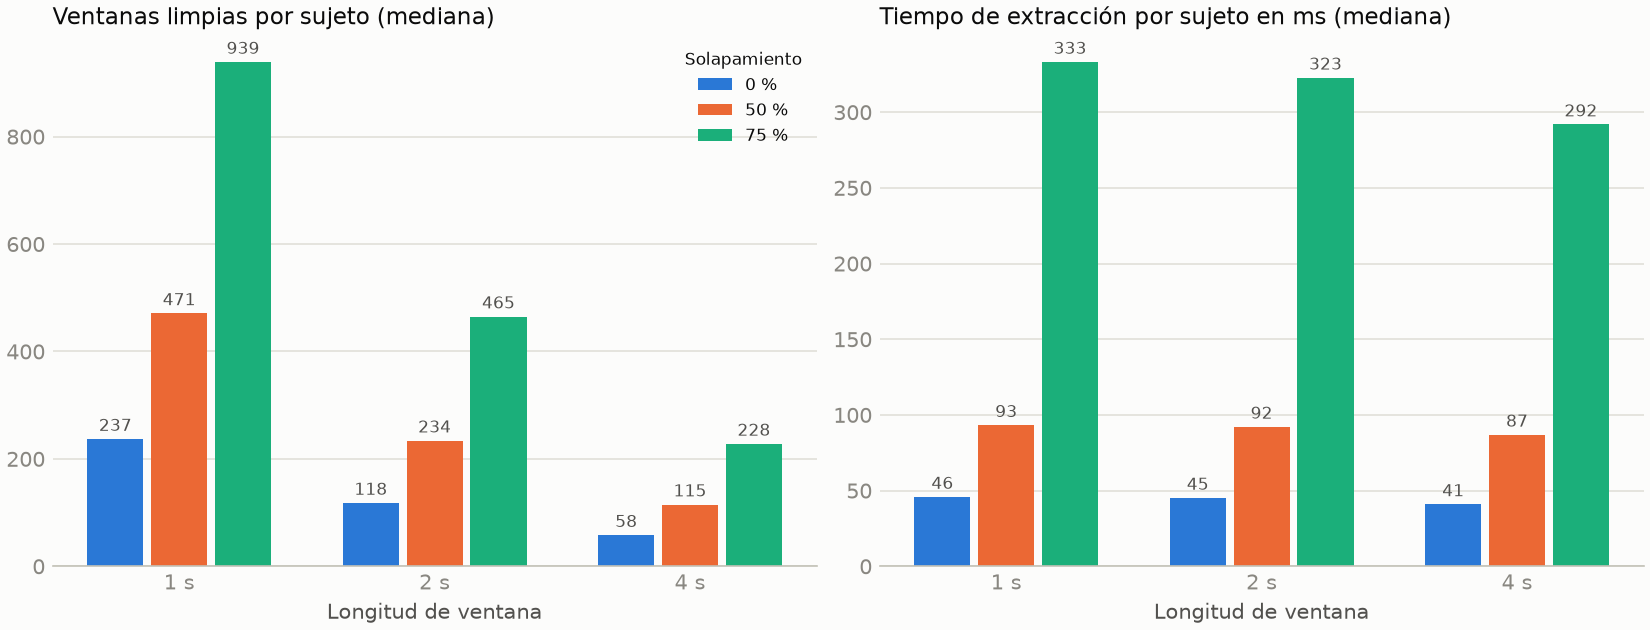
\includegraphics[width=0.95\textwidth]{fig_ventanas_tiempo.png}
\caption{Ventanas limpias y tiempo de extracción por sujeto (medianas) según la configuración.}
\label{fig:costo}
\end{figure}

% ---------------------------------------------------------------------------------------------
\section{Discusión preliminar}

\paragraph{El solapamiento no aporta estabilidad, solo costo.} Promediar ventanas solapadas reutiliza las mismas muestras, así que el promedio de cada sujeto casi no cambia. El ICC varió como mucho 0,02 en Alzheimer y depresión (0,07 en TEPT, con solo 12 sujetos), mientras que el tiempo se duplicó con 50~\% y se multiplicó por siete con 75~\%. Para el clasificador del paso~3, las ventanas solapadas aumentan el número de muestras pero no la información independiente; por eso es imprescindible validar por sujeto.

\paragraph{La longitud de ventana importa poco para la estabilidad del promedio, pero sí para otras cosas.} Fija la resolución en frecuencia (de 1 a 0,25~Hz), cambia el número de frecuencias de la entropía espectral y aumenta la pérdida de datos por artefactos (del 1--5~\% al 3--12~\% de las ventanas).

\paragraph{La prueba entre mitades está cerca de su techo.} Con 2 minutos por mitad, el promedio de decenas o cientos de ventanas borra casi todo el ruido de cada ventana individual, y el ICC queda alto en todas las configuraciones. Las diferencias entre configuraciones deberían aparecer a nivel de ventana individual, que es lo que verá el clasificador.

\paragraph{La amplitud puede ser un factor de confusión.} En TEPT y en depresión los pacientes tienen alrededor de la mitad de amplitud que los controles. Puede deberse a la enfermedad o al registro: en depresión, los archivos de controles y pacientes difieren incluso en sus canales auxiliares. Las características de potencia absoluta, que dependen de la amplitud, podrían separar a los grupos por motivos ajenos a la enfermedad. Conviene comparar los modelos con y sin ellas.

\paragraph{Implicación para trabajos como OnTEPT.} Para características promediadas por sujeto, la elección de ventana y solapamiento afecta poco a la fiabilidad pero mucho al costo, y cambia la resolución espectral. Documentar estos parámetros sigue siendo necesario para que los resultados sean reproducibles y comparables.

% ---------------------------------------------------------------------------------------------
\section{Limitaciones}
\begin{itemize}
  \item El conjunto de TEPT tiene solo 12 sujetos, se registró dentro de un resonador, llega preprocesado por sus autores y no se sabe si los participantes estaban en reposo.
  \item Se usan 240~s por sujeto para igualar la duración, de modo que en Alzheimer se descarta la mayor parte de cada registro.
  \item El rechazo de artefactos por umbral no detecta artefactos pequeños, como una contracción muscular leve.
  \item La banda gamma se limita a 30--40~Hz.
  \item El conjunto de depresión perdió 9 de sus 64 registros: 6 rotos en el repositorio, 2 duplicados y 1 demasiado corto.
  \item Las comparaciones entre conjuntos están confundidas por equipo, población y entorno; las comparaciones válidas son entre configuraciones dentro de cada conjunto.
  \item La estabilidad se mide entre dos mitades de la misma sesión, no entre sesiones de días distintos.
\end{itemize}

% ---------------------------------------------------------------------------------------------
\section{Trabajo pendiente}
\label{sec:pendiente}
El paso~3 consistirá en entrenar, en cada conjunto por separado, un clasificador simple de pacientes frente a controles para cada una de las nueve configuraciones:
\begin{itemize}
  \item Validación cruzada por sujeto, de modo que ningún sujeto tenga ventanas en entrenamiento y en prueba a la vez: dejando un sujeto fuera en TEPT, y con 5 particiones estratificadas por sujeto en Alzheimer y depresión.
  \item Estandarización de las características dentro de cada partición, ajustada solo con los sujetos de entrenamiento.
  \item Métricas a nivel de ventana y a nivel de sujeto.
  \item Interpretación con SHAP: qué características, bandas y canales pesan más, y si cambian entre configuraciones.
\end{itemize}
Quedan por decidir el tipo de clasificador (se propone regresión logística con regularización L2) y si se compara un modelo con todas las características frente a otro solo con las que no dependen de la amplitud.

\bibliographystyle{babunsrt-lf}
\bibliography{referencias}

% ---------------------------------------------------------------------------------------------
\appendix
\section{Resumen completo por configuración}

\begin{table}[ht]
\centering\small
\caption{Resultados por conjunto y configuración: ventanas limpias por sujeto (mediana), ventanas descartadas, tiempo de extracción por sujeto (mediana), ICC mediano de las 228 características y porcentaje de características con ICC $\ge$ 0,75.}
\label{tab:resumen}
\begin{tabular}{@{}lllrrrrr@{}}
\toprule
Conjunto & Ventana & Solap. & Ventanas & Descart. (\%) & Tiempo (ms) & ICC & ICC $\ge$ 0,75 (\%) \\
\midrule
\tabla{resumen.tex}
\bottomrule
\end{tabular}
\end{table}

\FloatBarrier
\section{Reproducibilidad}
Todo el código está en la carpeta del proyecto y se ejecuta con el entorno virtual \texttt{.venv}; las versiones exactas de las librerías están en \texttt{requirements.txt}.
\begin{itemize}
  \item \texttt{descargar\_datos.py}: descarga los datos a \texttt{datos/}, verifica tamaños y huellas MD5 y se puede reanudar.
  \item \texttt{paso2\_features.py}: armonización, ventanas, características, estabilidad y tiempos. Escribe en \texttt{resultados/paso2/} las características por ventana (27 archivos \texttt{.npz}), los CSV y las figuras de resultados.
  \item \texttt{material\_reporte.py}: figura de ejemplo y filas de las tablas de este informe, leídas de los CSV.
\end{itemize}
Orden de ejecución, desde la carpeta del proyecto:
\begin{verbatim}
.venv/bin/python -I descargar_datos.py
.venv/bin/python -I paso2_features.py
.venv/bin/python -I material_reporte.py
cd Report && latexmk -pdf reporte.tex
\end{verbatim}

\end{document}
